\documentclass[]{article}
\usepackage{lmodern}
\usepackage{amssymb,amsmath}
\usepackage{ifxetex,ifluatex}
\usepackage{fixltx2e} % provides \textsubscript
\ifnum 0\ifxetex 1\fi\ifluatex 1\fi=0 % if pdftex
  \usepackage[T1]{fontenc}
  \usepackage[utf8]{inputenc}
\else % if luatex or xelatex
  \ifxetex
    \usepackage{mathspec}
  \else
    \usepackage{fontspec}
  \fi
  \defaultfontfeatures{Ligatures=TeX,Scale=MatchLowercase}
\fi
% use upquote if available, for straight quotes in verbatim environments
\IfFileExists{upquote.sty}{\usepackage{upquote}}{}
% use microtype if available
\IfFileExists{microtype.sty}{%
\usepackage{microtype}
\UseMicrotypeSet[protrusion]{basicmath} % disable protrusion for tt fonts
}{}
\usepackage[unicode=true]{hyperref}
\hypersetup{
            pdfborder={0 0 0},
            breaklinks=true}
\urlstyle{same}  % don't use monospace font for urls
\usepackage{graphicx,grffile}
\makeatletter
\def\maxwidth{\ifdim\Gin@nat@width>\linewidth\linewidth\else\Gin@nat@width\fi}
\def\maxheight{\ifdim\Gin@nat@height>\textheight\textheight\else\Gin@nat@height\fi}
\makeatother
% Scale images if necessary, so that they will not overflow the page
% margins by default, and it is still possible to overwrite the defaults
% using explicit options in \includegraphics[width, height, ...]{}
\setkeys{Gin}{width=\maxwidth,height=\maxheight,keepaspectratio}
\IfFileExists{parskip.sty}{%
\usepackage{parskip}
}{% else
\setlength{\parindent}{0pt}
\setlength{\parskip}{6pt plus 2pt minus 1pt}
}
\setlength{\emergencystretch}{3em}  % prevent overfull lines
\providecommand{\tightlist}{%
  \setlength{\itemsep}{0pt}\setlength{\parskip}{0pt}}
\setcounter{secnumdepth}{0}
% Redefines (sub)paragraphs to behave more like sections
\ifx\paragraph\undefined\else
\let\oldparagraph\paragraph
\renewcommand{\paragraph}[1]{\oldparagraph{#1}\mbox{}}
\fi
\ifx\subparagraph\undefined\else
\let\oldsubparagraph\subparagraph
\renewcommand{\subparagraph}[1]{\oldsubparagraph{#1}\mbox{}}
\fi

% set default figure placement to htbp
\makeatletter
\def\fps@figure{htbp}
\makeatother


\date{}

\begin{document}

\emph{Sindrome del tunnel carpale}

Le sindromi canalicolari sono sindromi che coinvolgono sia l'arto
superiore che l'arto inferiore e sono caratterizzate dalla
\textbf{compressione di un nervo periferico all'interno di un canale
inestensibile}.

Nello specifico la sindrome del tunnel carpale è una delle più frequenti
dell'arto superiore ed è caratterizzata dalla compressione del
\emph{nervo mediano} a livello del tunnel carpale stesso.

L'innervazione motoria e sensitiva della mano è legata a tre nervi:

\begin{itemize}
\item
  \textbf{Nervo mediano:}
\end{itemize}

\begin{itemize}
\item
  INNERVAZIONE SENSITIVA: superficie palmare del primo, secondo, terzo e
  metà radiale del quarto dito.
\item
  INNERVAZIONE MOTORIA: muscoli dell'eminenza tenar.
\end{itemize}

\begin{itemize}
\item
  \textbf{Nervo ulnare:}
\end{itemize}

\begin{itemize}
\item
  INNERVAZIONE SENSITIVA: superficie palmare del quinto dito e metà
  ulnare del quarto dito.
\item
  INNERVAZIONE MOTORIA: muscoli dell'eminenza ipotenar.
\end{itemize}

\begin{itemize}
\item
  \textbf{Nervo radiale:}
\end{itemize}

\begin{itemize}
\item
  INNERVAZIONE SENSITIVA: dorso della mano.
\end{itemize}

Definizione

La sindrome del tunnel carpale è stata scoperta nel 1913 da Marie e
Foix.

Il primo intervento di decompressione è stato svolto presso la Mayo
Clinic da Galloway nel 1924.

Può essere definita come l'insieme dei sintomi e dei segni conseguenti
alla compressione del nervo mediano nel passaggio all'interno del tunnel
carpale.

Il \textbf{canale carpale} è un canale osteo-fibroso inestensibile,
localizzato tra palmo della mano e polso, attraverso il quale decorrono
il \emph{nervo mediano} e i \emph{9} (4 superficiali e 5 profondi)
\emph{tendini flessori} per le dita della mano.

È costituito da:

\begin{itemize}
\item
  un PAVIMENTO concavo, composto dalle ossa carpali
\item
  un TETTO fibroso, formato dal \emph{legamento trasverso del carpo}.
\end{itemize}

\emph{Il \textbf{\emph{tunnel carpale}}, è definito come quel canale
osteofibroso che ha come pavimento l'estremità distale di radio ed ulna,
lo scafoide, il piramidale ed il pisiforme, come tetto il legamento
trasverso del carpo, come parete laterale i tubercoli dello scafoide e
del trapezio e come parete mediale il pisiforme ed l'uncino
dell'uncinato.} \emph{All'interno del canale decorrono diverse
strutture, nello specifico troviamo il \textbf{\emph{nervo mediano}}, in
posizione alquanto superficiale, i \emph{tendini dei muscoli flessori
superficiale e profondo delle dita}, il \emph{tendine del flessore lungo
del pollice} e diversi vasi sanguigni.}

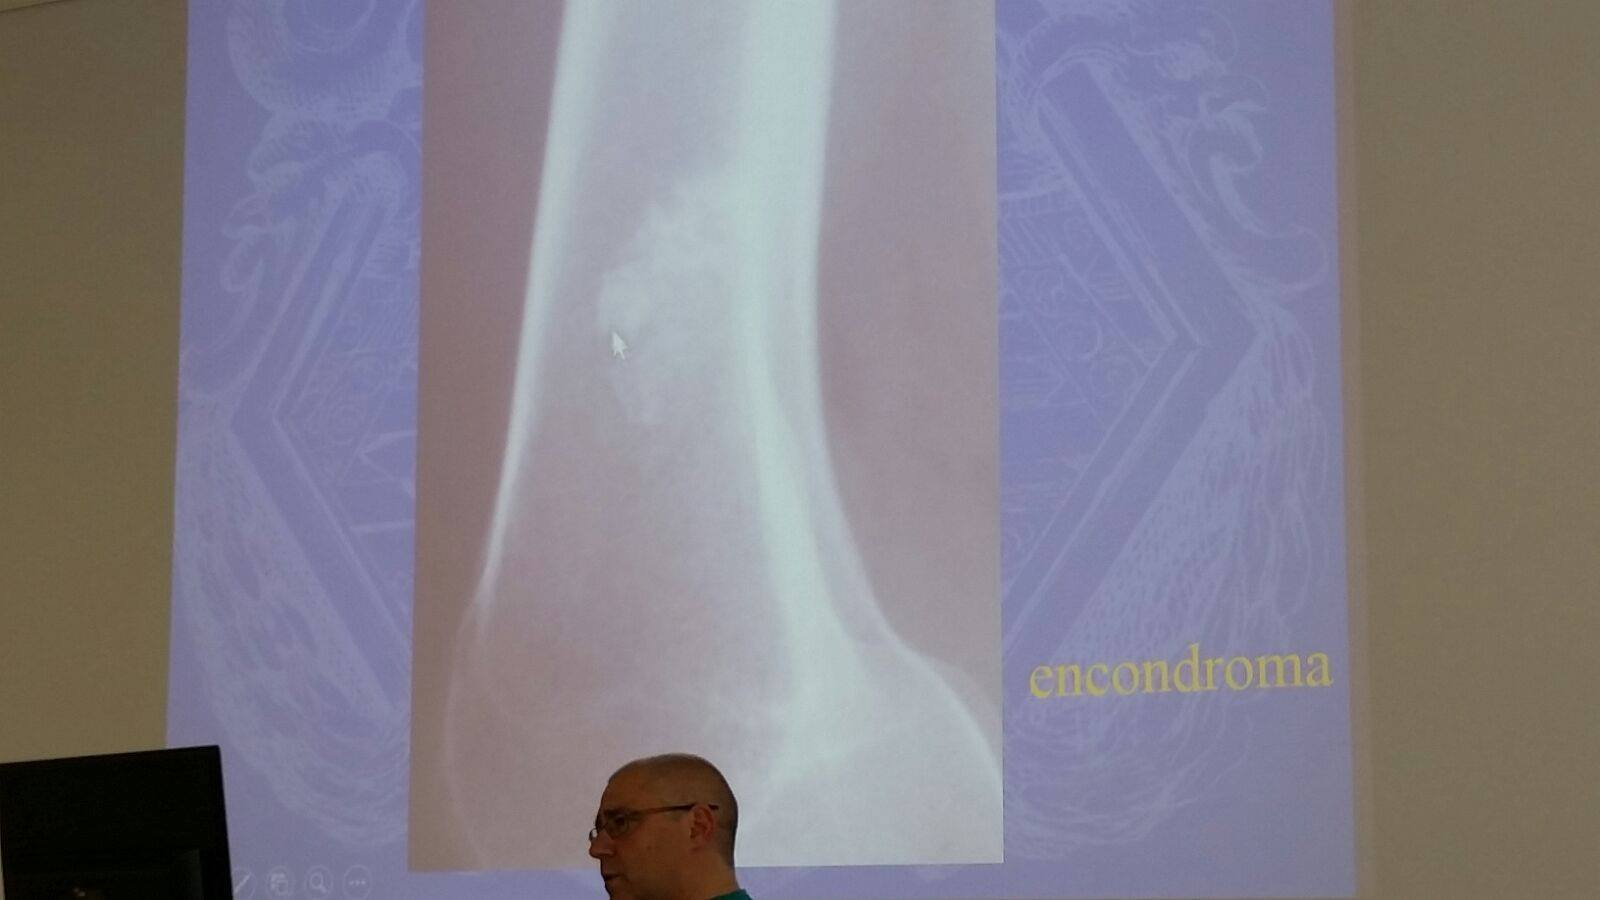
\includegraphics[width=3.41667in,height=2.49653in]{media/image1.jpeg}

La sintomatologia è dovuta ad un \textbf{aumento pressorio} all'interno
di questo canale inestensibile (da alcuni studi si è visto che si può
passare da 2,5 mmHg a più di \textbf{30 mmHg}).

Due posizioni (flessione palmare e dorsale) aumentano molto la pressione
all'interno del canale carpale, soprattutto in questo tipo di patologia,
e sono utilizzate come test specifici per fare diagnosi della patologia.

Cause

Le cause di aumento pressorio all'interno del tunnel carpale sono tutte
quelle condizioni che portano a:

\begin{itemize}
\item
  ESPANSIONE del contenuto del canale
\item
  RESTRINGIMENTO di ciò che sta attorno al tunnel carpale.
\end{itemize}

Tra le varie cause troviamo:

\begin{itemize}
\item
  ispessimento del legamento trasverso del carpo
\item
  processo infiammatorio tendineo e peritendineo dei tendini flessori
  (una delle cause più frequenti)
\item
  neoformazioni, lipomi, cisti all'interno del canale carpale
\item
  frammento osseo di frattura che schiaccia il nervo
\item
  callo osseo esuberante dopo una frattura di polso
\item
  osteofiti derivanti da malattie degenerative
\item
  deposizione sostanze patologiche (come in gotta, amiloidosi,
  insufficienza renale,\ldots{})
\item
  tumori intraneurali (neurinomi del nervo mediano)
\end{itemize}

\emph{Epidemiologia }

\begin{itemize}
\item
  E' più frequente nel sesso femminile, spesso in età perimenopausale
  (40-60 anni).
\item
  Il sesso maschile è meno coinvolto: riguarda perlopiù soggetti con
  attività lavorative che comportano prese di forza, movimenti ripetuti
  o uso di strumenti vibranti.
\item
  Nella maggior parte dei casi è colpito il lato dominante, ma ci può
  anche essere una bilateralità.
\item
  Può essere isolata o associata ad altre patologie della mano:
  \textbf{sindrome di De Quervain}, \textbf{dito a scatto},
  \textbf{rizartrosi}.
\end{itemize}

\emph{Eziopatogenesi }

\begin{itemize}
\item
  Idiopatica
\item
  Secondarie:
\end{itemize}

\begin{itemize}
\item
  Le condizioni già viste che causano aumento di pressione
\item
  Condizioni che aumentano la \emph{suscettibilità del nervo} (come il
  diabete o \emph{anomalie congenite} del nervo mediano stesso, ad
  esempio il nervo mediano bipartito, che aumentano la suscettibilità
  del nervo stesso).
\end{itemize}

\begin{itemize}
\item
  Forme acute come quelle post-traumatiche.
\item
  La causa più frequente che riduce lo spazio è la \emph{TENOSINOVITE
  DEI FLESSORI} che vanno a schiacciare il nervo mediano.
\item
  \emph{Può poi essere dovuta o a una condizione di
  \textbf{\emph{aumento del volume del contenuto del canale}} (ad
  esempio per \emph{cisti sinoviali} o \emph{infiammazione delle guaine
  tendinee}, ma anche per \emph{tumori} o per altre \emph{patologie
  espansive}) oppure una \textbf{\emph{riduzione delle dimensioni del
  tunnel stesso}}, che può essere dovuta o ad \emph{esiti di fratture
  del polso} guarite con un vizio di consolidazione, o anche ad una
  \emph{tenovaginite cronica ipertrofica}, la quale è nella maggior
  parte dei casi idiopatica e legata probabilmente anche ad alcuni
  \textbf{fattori ormonali} (in particolare il calo degli estrogeni) e
  ai \textbf{microtraumatismi} (come le attività lavorative con prese di
  forza o movimenti ripetitivi del polso), mentre più raramente la causa
  è \textbf{\emph{reumatologica}}.}
\end{itemize}

Ci sono patologie che favoriscono l'insorgenza del tunnel carpale :

\begin{itemize}
\item
  diabete
\item
  patologie tiroidee
\item
  iperaldosteronismo
\item
  Insufficienza renale cronica
\item
  gravidanza e allattamento (che, anche se non sono condizioni
  patologiche, sono comunque predisponenti all'insorgenza della
  sindrome. A fine gravidanza e allattamento la sintomatologia recede)
\end{itemize}

In queste patologie (diabete, patologie tiroidee, iperaldosteronismo),
l'esito dipende dal trattamento della patologia di base, perciò bisogna
sempre dire al paziente che il recupero potrebbe non essere completo se
il nervo è già rovinato dalla sottostante patologia.

\begin{itemize}
\item
  Bisogna prestare attenzione anche agli scoagulati.
\item
  Bisogna sempre aprire un gesso che dà fastidio, perché se troppo
  stretto potrebbe dare una compressione nervosa.
\item
  Lussazione delle ossa carpali possono dare compressione.
\item
  Trombosi dell'arteria (raro)
\end{itemize}

Ricapitolando, le cause più frequenti di compressione sono :

\begin{itemize}
\item
  ISPESSIMENTO LEGAMENTO TRASVERSO DEL CARPO
\item
  PROCESSO ESPANSIVO/INFIAMMATORIO DEI TENDINI FLESSORI CHE PASSANO
  ALL'INTERNO DEL TUNNEL CARPALE
\end{itemize}

\emph{Diagnosi}

Nella maggior parte dei casi si presenta una signora (perché appunto le
femmine sono maggiormente colpite rispetto ai maschi ), che di notte si
sveglia alla stessa ora perché si sente la mano pesante e addormentata
nella zona di innervazione del nervo mediano.

Quindi, dopo aver scrollato la mano per 1-2 minuti, questa sensazione
passa e la paziente si riaddormenta.

Durante il giorno questa sintomatologia ritorna soprattutto in movimenti
di \emph{presa statica} (quando si guida, si va in bici), con
\textbf{formicolii} simili alla sintomatologia notturna, spesso
associati a sensazione di \textbf{tumefazione}.

Ci può essere \textbf{dolore} fino alla radice delle dita o che risale
fino al gomito ed alla spalla (irradiazione prossimale).

Al mattino c'è una maggiore rigidità dell'articolazione.

D'inverno i sintomi si verificano molto più frequentemente che d'estate.

Negli stadi avanzati queste sensazioni di alterata sensibilità e di
dolore diventano costanti e si può arrivare all'\textbf{ipotrofia
dell'eminenza tenar} con difficoltà nello svolgimento di movimenti fini
delle dita (in passato le donne riferivano l'impossibilità di cucire).

Il dolore con il tempo tende a scomparire.

Di solito i sintomi sensitivi anticipano quelli motori (è raro che
avvenga il contrario).

Il decorso di solito non è particolarmente veloce, anche se in alcuni
casi (ad esempio negli anziani e nei diabetici, dove ci possono essere
altre neuropatie) l'insorgenza è acuta e si aggrava velocemente.

\emph{Obiettività }

Bisogna innanzitutto osservare la mano e ricercare:

\begin{itemize}
\item
  Eventuali deformità
\item
  Ipotrofia dell'eminenza tenar
\item
  Se il paziente riesce ad effettuare il movimento di opposizione
  (controllato dal ramo motorio del n. mediano)
\end{itemize}

Esistono dei test neurologici come:

\begin{itemize}
\item
  Test di discriminazione di due punti statici (di Weber)
\item
  Test di soglia
\item
  Valutare se ci sono deficit motori, osservando l'abduttore breve e
  l'opponente del pollice e il flessore breve delle dita.
\end{itemize}

Si fanno poi dei test provocativi :

\begin{itemize}
\item
  \emph{Test di Tinel}: percussione a livello del passaggio del nervo
  mediano nel canale carpale. È positivo se c'è una sensazione di scossa
  nella zona di innervazione del nervo mediano
\item
  \emph{Test di Phalen normale}: si chiede al paziente di mettere le
  mani dorso contro dorso, tenendo i gomiti a 90 gradi. E' positivo se
  entro 60 secondi compare formicolio anche intenso se il nervo mediano
  è compresso.
\end{itemize}

\begin{quote}
\emph{\emph{Nb: è bene tenere a mente che questi due test sono
sicuramente positivi nelle prime fasi, mentre in fase paralitica possono
anche risultare negativi.}}
\end{quote}

\begin{itemize}
\item
  \emph{Test di Phalen inverso}: c'è una flessione dorsale della mano e,
  anche in questo caso, è positivo se il paziente avverte formicolio
  entro 60 secondi nella zona di innervazione del nervo mediano
\item
  \emph{Test di Durkan}: si schiaccia il nervo in corrispondenza del
  tunnel carpale. Di solito è positivo se compaiono i sintomi dopo 30
  secondi dalla compressione.
\end{itemize}

\textbf{Diagnosi differenziale:}

\begin{itemize}
\item
  Una compressione C5-C6 del rachide, che presenta una sintomatologia
  simile.
\item
  Alcune patologie neurologiche possono dare sintomi simili, quindi
  bisogna fare attenti esami neurologici.
\item
  Considerare sempre il diabete, che può avere una neuropatia di base.
\end{itemize}

\emph{Esami strumentali}

L'\emph{elettromiografia} è un esame elettrofisiologico in cui si
applicano delle scosse prossimalmente al livello della compressione e si
registra la velocità di propagazione dell'impulso→ se è bassa vuol dire
che c'è la compressione del nervo.

Permette quindi di rilevare il \textbf{grado} di compressione del nervo
e quanto è grave questa compromissione. Rileva anche la
\textbf{localizzazione} della compressione del nervo: se la compressione
è prossimale (a livello del gomito) o se è distale, a livello del polso.

Questo è un aiuto importante dal punto di vista della scelta terapeutica
e nel post-operatorio una rivalutazione elettromiografica permette di
capire se l'intervento è riuscito.

L'\emph{ecografia} è un altro esame che si può fare. È un esame di
supporto, però molto meno usato rispetto all'elettromiografia. Usata in
caso di sospette lesioni ai tessuti molli.

L\emph{'Rx} è utile solo in esiti di patologie ossee.

\emph{Classificazione Clinica }

A seconda del grado di compressione del nervo si distinguono:

\begin{enumerate}
\def\labelenumi{\arabic{enumi}.}
\item
  Fase \textbf{algico-irritativa:} in cui il nervo è neuroaprassico. Ci
  possono essere dei fastidi. \emph{Fase caratterizzata da parestesie
  prevalentemente notturne in corrispondenza della superficie palmare
  delle prime 3 dita della mano e della metà del quarto dito, cioè in
  quella che è l'area di innervazione del nervo mediano.}
\item
  Fase \textbf{parestesico-dolorosa:} in cui il nervo è più compresso,
  con alcune degenerazioni. \emph{Ai sintomi della fase precedente si
  associano anche \emph{ipovalidità} ed \emph{ipotrofia dei muscoli
  dell'eminenza tenar} (opponente del pollice, abduttore breve del
  pollice e capo superficiale del flessore breve del pollice) \emph{e
  dei primi due lombricali}, con anche ipoestesia nel territorio di
  innervazione e difficoltà nel controllo della presa degli oggetti}
\item
  Fase \textbf{atrofico-paralitica:} è la fase finale, la più grave,
  caratterizzata anche da disturbi motori. \emph{\emph{Marcata atrofia
  dei muscoli dell'eminenza tenar associata ad ipoanestesia delle prime
  3 dita e della metà del quarto, con abolizione del movimento di
  opposizione del pollice.}}
\end{enumerate}

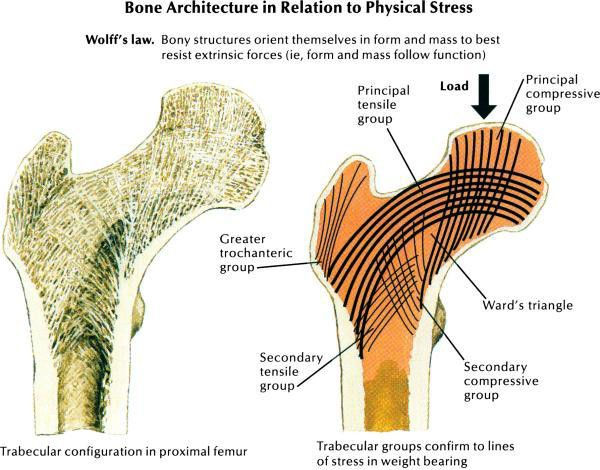
\includegraphics[width=3.93750in,height=3.09861in]{media/image2.jpeg}

Le fasi 1 e 2 sono reversibili con il trattamento.

Nella fase 3, anche se si va ad intervenire con un intervento
chirurgico, sarà molto difficile avere una restitutio ad integrum: ci
saranno dei miglioramenti dal punto di vista sintomatologico, ma non ci
sarà miglioramento dal punto di vista della forza e dell'atrofia del
muscolo.

\emph{Il recupero sarà tanto più veloce tanto più è stata breve la
compressione e sarà tanto più completo quanto meno grave è stata la
compressione.}

\emph{Trattamento}

\begin{itemize}
\item
  \textbf{Conservativo} (Stadi 1 e 2): nello stadio 1 si possono fare
  delle \emph{infiltrazioni di corticosteroidi} (massimo due all'anno)
  all'interno del canale carpale, attorno al nervo e ai tendini che
  molto spesso sono infiammati.
\end{itemize}

\begin{quote}
Si possono fare anche \emph{terapie fisiche}.

Ma soprattutto ha un effetto positivo il trattamento con \emph{tutori}
(solo di notte o giorno e notte) che evitano posizioni di iperestensione
e di iperflessione che aumenterebbero la pressione nel canale. Essi
immobilizzano il polso in \emph{posizione neutra} (2-9º in flessione
dorsale, 2-6º di deviazione ulnare), in cui il nervo è stressato al
minimo.
\end{quote}

\begin{itemize}
\item
  Nello stadio 2 e 3 (o qualora il trattamento conservativo non abbia
  avuto effetto) si può arrivare al \textbf{trattamento chirurgico}:
  consiste nell'apertura del tunnel carpale attraverso la \emph{sezione
  del legamento trasverso del carpo} senza danneggiare il nervo mediano
  che sta sotto. E' effettuato in anestesia locale, quindi in regime
  ambulatoriale.
\end{itemize}

\begin{quote}
Si può fare:
\end{quote}

\begin{itemize}
\item
  \emph{a cielo aperto} attraverso l'incisione classica: incisione del
  palmo della mano lungo l'asse del quarto dito, si scolla cute e
  sottocute e si seziona longitudinalmente il legamento trasverso del
  carpo. Una volta sezionato, sotto si trova il nervo e attorno i
  tendini: se il nervo è troppo compresso si può fare una
  \textbf{neurolisi}, cioè si libera il nervo dalle aderenze e a volte
  si toglie anche la sinovia che infiamma il tendine.
\end{itemize}

\begin{quote}
{[}Per differenziare \emph{nervi e tendini, basta piegare passivamente
le dita: il nervo resta fisso mentre} i tendini scorrono{]}.

Si possono anche fare delle mini incisioni a livello del polso e del
palmo della mano, si passa sotto con una sonda e si seziona per via
sottocutanea.
\end{quote}

\begin{itemize}
\item
  per via endoscopica che offre minori tempi di recupero ma con un
  maggior rischio di complicanze intraoperatorie.
\end{itemize}

\emph{In ogni caso, il trattamento chirurgico garantisce un netto
miglioramento del dolore ed un buon recupero sensitivo e motorio, purché
si sia andati ad agire tempestivamente (infatti più a lungo il nervo
rimane compresso e tanto minore sarà il recupero, fino ad essere del
tutto assente).}

\emph{Post-operatorio}

In genere si esegue un \textbf{bendaggio} o si utilizza un
\textbf{tutore}.

Si dice al paziente di muovere le dita e di tenere in alto la mano
affinché non si provochino ematomi.

Dopo 2 settimane si tolgono i punti ed inizia la cura della cicatrice,
che può dar fastidio per 1-2 mesi. Si consigliano \emph{massaggi} (2-3
volte al giorno per una ventina di giorni) per far passare il fastidio
legato alla cicatrice.

Si possono associare anche \emph{ultrasuoni}.

È necessario avvisare il paziente che non ritornerà subito completamente
alla manualità precedente perché i tempi di pieno recupero sono di circa
1-2 mesi.

\emph{Complicanze}

Può sembrare un intervento banale ma il rischio più grave è il
\textbf{taglio della branca motoria del nervo mediano.} Essa normalmente
si sfiocca oltre il legamento trasverso mediano.

Ci possono però essere delle varianti anatomiche in cui si sfiocca al di
sotto o dentro il legamento trasverso: per questo nel sezionare è meglio
portarsi verso il lato ulnare piuttosto che direttamente sopra il nervo.

Ovviamente non bisogna stare troppo sul lato ulnare perché si rischia di
lesionare il nervo ulnare.

Altra complicazione può essere la recidiva per cicatrizzazione ed
inspessimento del legamento trasverso del carpo.

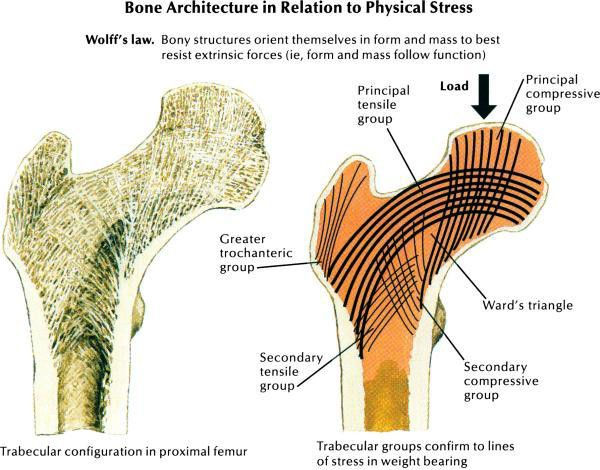
\includegraphics[width=5.68819in,height=2.34375in]{media/image3.jpeg}

\emph{Altri siti di compressione dei nervi nell'arto superiore }

\emph{Nervo Ulnare}

Può avere 2 siti di compressione:

\begin{itemize}
\item
  a livello della \textbf{doccia epitrocleolecranica} del gomito.
\end{itemize}

SINTOMI: intorpidimento lungo la zona di innervazione sensitiva del
nervo ulnare e nei casi gravi ipotrofia dell'eminenza tenar.

\begin{itemize}
\item
  \textbf{Sindrome del canale di Guyon} se è compresso a livello del
  polso.
\end{itemize}

\emph{Nervo Mediano}

\begin{itemize}
\item
  A livello del \textbf{canale carpale}
\item
  \textbf{Sindrome del nervo INTEROSSEO ANTERIORE:} quando compresso
  nella sua branca motoria a livello del gomito.
\end{itemize}

\begin{quote}
SINTOMI: prevalentemente motori, a livello dei muscoli dell'avambraccio.
\end{quote}

\emph{Nervo Radiale}

\begin{itemize}
\item
  Può essere lesionato e stirato nelle fratture del terzo distale
  dell'omero
\item
  \textbf{Compressione del} \textbf{nervo INTEROSSEO POSTERIORE:}
  compressione della sua componente motoria, che innerva i muscoli
  estensori delle dita.
\item
  Compressioni più alte a livello sottoclavicolare (legate per esempio
  ad una sindrome dello sbocco toracico).
\end{itemize}

\emph{Patologie compressive nell'arto inferiore}

\begin{itemize}
\item
  \textbf{Sindrome del tunnel tarsale:} è il corrispettivo, a livello
  del piede, della sindrome del tunnel carpale. Consiste nella
  compressione del \emph{nervo tibiale posteriore} a livello della
  doccia retromalleolare mediale.
\end{itemize}

SINTOMI: formicolii a livello della pianta del piede.

\begin{itemize}
\item
  \textbf{Compressione del nervo sciatico popliteo} \textbf{esterno} a
  livello della testa del perone (particolarmente vero nelle forme acute
  delle fratture del piatto tibiale oppure nelle forme acute nel caso di
  pazienti allettati da molto tempo e che tendono ad avere la gamba
  extra ruotata, per cui il nervo può essere schiacciato, ma ci sono
  anche forme idiopatiche).
\item
  \textbf{Sindrome del piriforme:} è una sindrome per esclusione (nello
  sportivo soprattutto), da compressione del nervo sciatico dal bordo
  inferiore del muscolo piriforme. Il nervo sciatico può essere
  lesionato o compresso quando si ha una lussazione dell'anca.
\item
  Il \textbf{nervo femorale} a volte può essere stirato quando si fa un
  accesso laterale all'anca: uno stiramento da parte dei divaricatori
  può essere presente nella artrosi concentriche dell'anca.
\end{itemize}

\end{document}
